\documentclass[14pt]{extbook}
\usepackage{multicol, enumerate, enumitem, hyperref, color, soul, setspace, parskip, fancyhdr} %General Packages
\usepackage{amssymb, amsthm, amsmath, latexsym, units, mathtools} %Math Packages
\everymath{\displaystyle} %All math in Display Style
% Packages with additional options
\usepackage[headsep=0.5cm,headheight=12pt, left=1 in,right= 1 in,top= 1 in,bottom= 1 in]{geometry}
\usepackage[usenames,dvipsnames]{xcolor}
\usepackage{dashrule}  % Package to use the command below to create lines between items
\newcommand{\litem}[1]{\item#1\hspace*{-1cm}\rule{\textwidth}{0.4pt}}
\pagestyle{fancy}
\lhead{Progress Quiz 7}
\chead{}
\rhead{Version A}
\lfoot{4173-5738}
\cfoot{}
\rfoot{Spring 2021}
\begin{document}

\begin{enumerate}
\litem{
Choose the equation of the function graphed below.
\begin{center}
    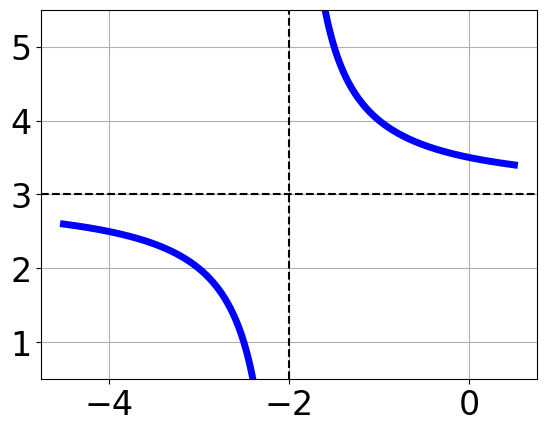
\includegraphics[width=0.5\textwidth]{../Figures/rationalGraphToEquationA.png}
\end{center}
\begin{enumerate}[label=\Alph*.]
\item \( f(x) = \frac{-1}{x - 3} + 1 \)
\item \( f(x) = \frac{1}{(x + 3)^2} + 1 \)
\item \( f(x) = \frac{1}{x + 3} + 1 \)
\item \( f(x) = \frac{-1}{(x - 3)^2} + 1 \)
\item \( \text{None of the above} \)

\end{enumerate} }
\litem{
Determine the domain of the function below.\[ f(x) = \frac{3}{15x^{2} -43 x + 30} \]\begin{enumerate}[label=\Alph*.]
\item \( \text{All Real numbers.} \)
\item \( \text{All Real numbers except } x = a, \text{ where } a \in [0.92, 1.5] \)
\item \( \text{All Real numbers except } x = a \text{ and } x = b, \text{ where } a \in [14.93, 15.92] \text{ and } b \in [29.84, 30.14] \)
\item \( \text{All Real numbers except } x = a, \text{ where } a \in [14.93, 15.92] \)
\item \( \text{All Real numbers except } x = a \text{ and } x = b, \text{ where } a \in [0.92, 1.5] \text{ and } b \in [1.45, 1.75] \)

\end{enumerate} }
\litem{
Solve the rational equation below. Then, choose the interval(s) that the solution(s) belongs to.\[ \frac{-3x}{7x + 4} + \frac{-4x^{2}}{-35x^{2} -34 x -8} = \frac{6}{-5x -2} \]\begin{enumerate}[label=\Alph*.]
\item \( x \in [-0.53,-0.24] \)
\item \( x_1 \in [-0.72, -0.48] \text{ and } x_2 \in [-6.57,0.43] \)
\item \( x_1 \in [-0.72, -0.48] \text{ and } x_2 \in [2.84,4.84] \)
\item \( \text{All solutions lead to invalid or complex values in the equation.} \)
\item \( x \in [3.52,4.22] \)

\end{enumerate} }
\litem{
Determine the domain of the function below.\[ f(x) = \frac{5}{9x^{2} -9} \]\begin{enumerate}[label=\Alph*.]
\item \( \text{All Real numbers except } x = a, \text{ where } a \in [-10.8, -8.2] \)
\item \( \text{All Real numbers except } x = a \text{ and } x = b, \text{ where } a \in [-1.6, -0.5] \text{ and } b \in [-0.2, 1.2] \)
\item \( \text{All Real numbers except } x = a, \text{ where } a \in [-1.6, -0.5] \)
\item \( \text{All Real numbers.} \)
\item \( \text{All Real numbers except } x = a \text{ and } x = b, \text{ where } a \in [-10.8, -8.2] \text{ and } b \in [8.9, 10] \)

\end{enumerate} }
\litem{
Choose the graph of the equation below.\[ f(x) = \frac{1}{x - 2} + 1 \]\begin{enumerate}[label=\Alph*.]
\begin{multicols}{2}\item 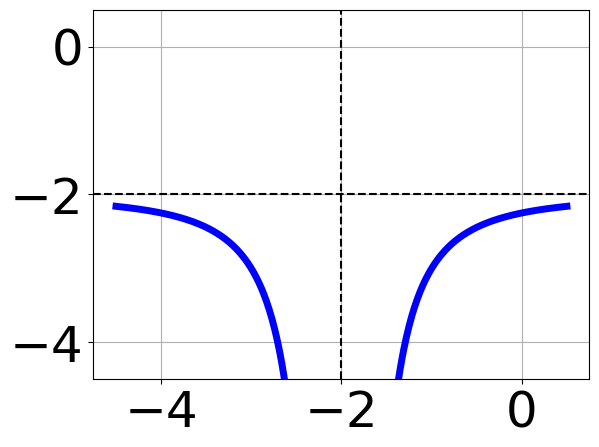
\includegraphics[width = 0.3\textwidth]{../Figures/rationalEquationToGraphAA.png}\item 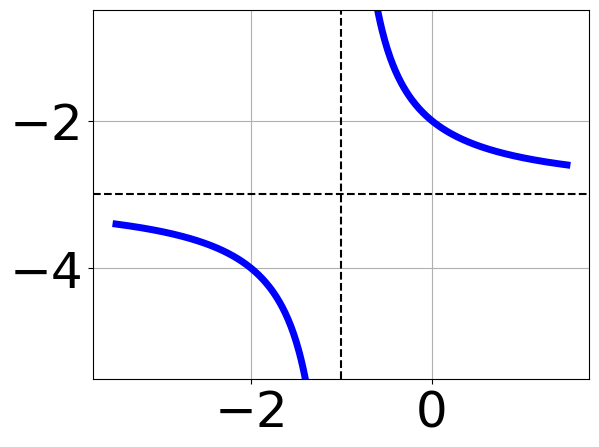
\includegraphics[width = 0.3\textwidth]{../Figures/rationalEquationToGraphBA.png}\item 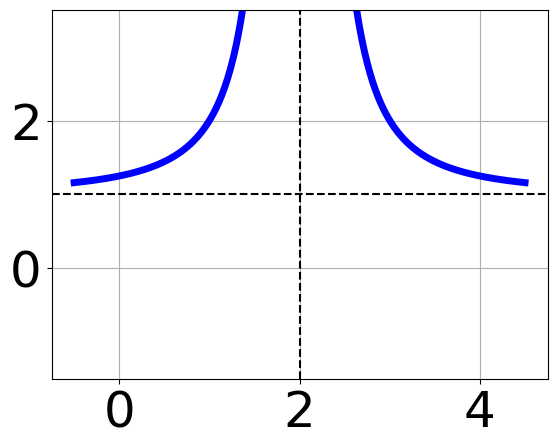
\includegraphics[width = 0.3\textwidth]{../Figures/rationalEquationToGraphCA.png}\item 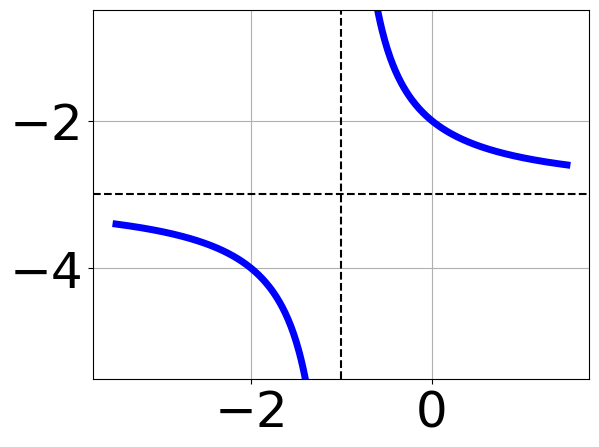
\includegraphics[width = 0.3\textwidth]{../Figures/rationalEquationToGraphDA.png}\end{multicols}\item None of the above.
\end{enumerate} }
\litem{
Choose the equation of the function graphed below.
\begin{center}
    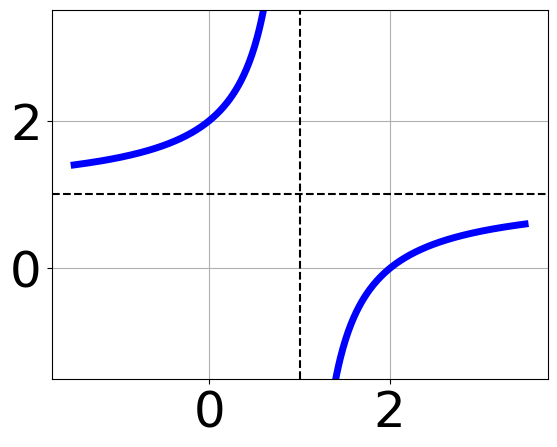
\includegraphics[width=0.5\textwidth]{../Figures/rationalGraphToEquationCopyA.png}
\end{center}
\begin{enumerate}[label=\Alph*.]
\item \( f(x) = \frac{-1}{x - 2} + 3 \)
\item \( f(x) = \frac{-1}{(x - 2)^2} + 3 \)
\item \( f(x) = \frac{1}{(x + 2)^2} + 3 \)
\item \( f(x) = \frac{1}{x + 2} + 3 \)
\item \( \text{None of the above} \)

\end{enumerate} }
\litem{
Choose the graph of the equation below.\[ f(x) = \frac{-1}{(x + 3)^2} - 1 \]\begin{enumerate}[label=\Alph*.]
\begin{multicols}{2}\item 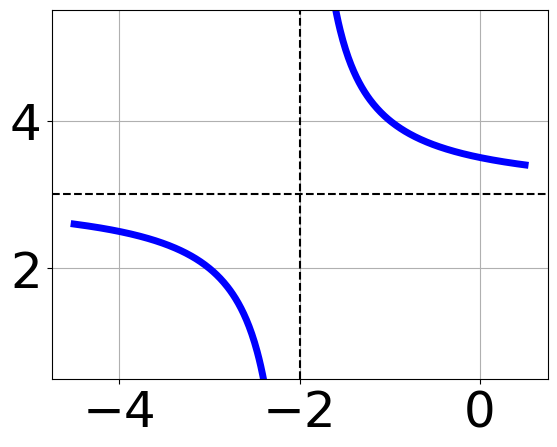
\includegraphics[width = 0.3\textwidth]{../Figures/rationalEquationToGraphCopyAA.png}\item 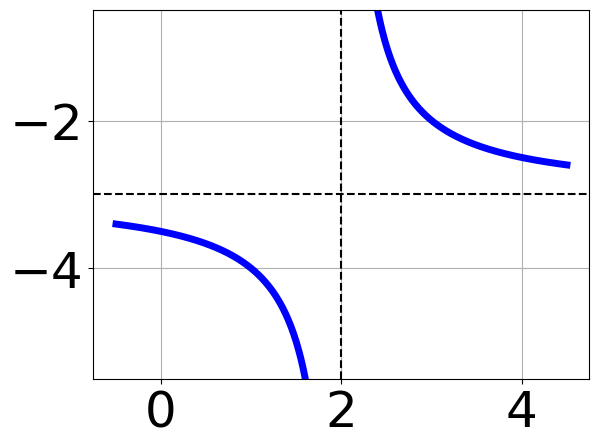
\includegraphics[width = 0.3\textwidth]{../Figures/rationalEquationToGraphCopyBA.png}\item 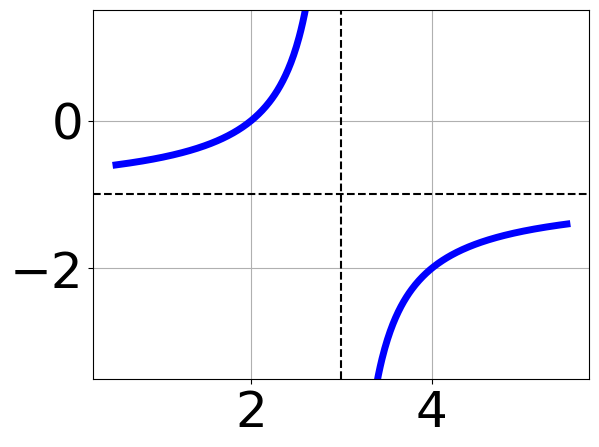
\includegraphics[width = 0.3\textwidth]{../Figures/rationalEquationToGraphCopyCA.png}\item 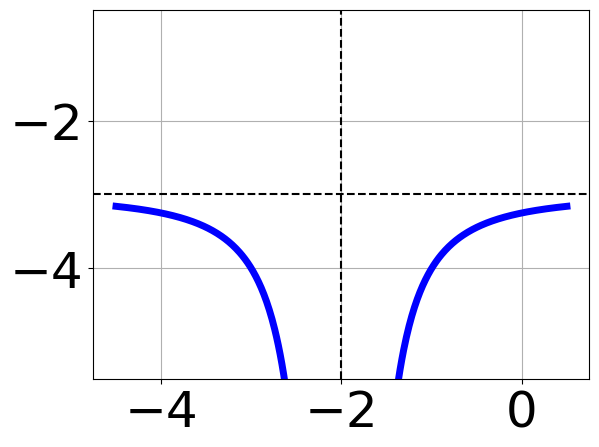
\includegraphics[width = 0.3\textwidth]{../Figures/rationalEquationToGraphCopyDA.png}\end{multicols}\item None of the above.
\end{enumerate} }
\litem{
Solve the rational equation below. Then, choose the interval(s) that the solution(s) belongs to.\[ \frac{-5}{-4x + 8} + 2 = \frac{9}{-8x + 16} \]\begin{enumerate}[label=\Alph*.]
\item \( x \in [-3.59,-2.59] \)
\item \( x_1 \in [-0.18, 0.28] \text{ and } x_2 \in [0.81,3.81] \)
\item \( x_1 \in [-3.59, -2.59] \text{ and } x_2 \in [0.81,3.81] \)
\item \( x \in [0.81,1.81] \)
\item \( \text{All solutions lead to invalid or complex values in the equation.} \)

\end{enumerate} }
\litem{
Solve the rational equation below. Then, choose the interval(s) that the solution(s) belongs to.\[ \frac{-7x}{-5x -3} + \frac{-2x^{2}}{10x^{2} -14 x -12} = \frac{-6}{-2x + 4} \]\begin{enumerate}[label=\Alph*.]
\item \( x \in [1.3,2.4] \)
\item \( x \in [4.6,6] \)
\item \( x_1 \in [-0.9, 0.7] \text{ and } x_2 \in [2.13,6.13] \)
\item \( x_1 \in [-0.9, 0.7] \text{ and } x_2 \in [-0.6,1.4] \)
\item \( \text{All solutions lead to invalid or complex values in the equation.} \)

\end{enumerate} }
\litem{
Solve the rational equation below. Then, choose the interval(s) that the solution(s) belongs to.\[ \frac{56}{14x -63} + 1 = \frac{56}{14x -63} \]\begin{enumerate}[label=\Alph*.]
\item \( x \in [-4.5,-3.5] \)
\item \( x_1 \in [-4.5, -3.5] \text{ and } x_2 \in [2.5,8.5] \)
\item \( x_1 \in [3.5, 5.5] \text{ and } x_2 \in [2.5,8.5] \)
\item \( \text{All solutions lead to invalid or complex values in the equation.} \)
\item \( x \in [4.5,5.5] \)

\end{enumerate} }
\end{enumerate}

\end{document}